\chapter{Evaluación Experimental}\label{chap:evaluacion}

En este capitulo de expondrá los resultados que se obtuvieron por medio de los experimentos realizados. Los pasos seguidos serán presentados dividiendo en diferentes secciones para lograr una mayor comprensión en el trabajo.

La primera sección \textit{Preparación de Datos} \ref{sec:preparacion_de_datos}, se muestran cuales fueron los datos finales para realizar los experimentos.

La segunda parte  \textit{Selección de modelos y Clasificación}, se detallan los modelos y clasificadores utilizados en la experimentación.

Para finalizar  la sección \textit{validación} detallamos los resultados finales obtenidos.


\section{Preparación de Datos}\label{sec:preparacion_de_datos}

Vamos a partir de las imágenes obtenidas en el capitulo \ref{chap:recoleccion} donde se puso en detalle los tipos de imágenes que serán utilizadas. En esta sección hablaremos de cual es el \textit{ground truth}, región verdadera, utilizada; como se realizo la extracción de característica de cada imagen, y que criterio de selección de candidatos se utilizo para el entrenamiento.

\subsection{Ground truth}\label{sub:groundtruth}

El problema abordado es un problema de clasificación supervisada, es por esto que debemos saber anticipadamente donde se encuentra el objeto de interés que deseamos detectar. En \ac{ml} el termino \textit{ground truth} hace referencia a la información provenida desde la observación; \textit{ground truth} involucra a un conjunto de imágenes y un conjunto de etiquetas en las imágenes que incluye la locación y las características claves en la imagen.

Las etiquetas se añadieron manualmente utilizando una librería desarrollada en python llamada \textit{labelme}\footnote{Fuente: 
https://github.com/wkentaro/labelme}; que nos permite realizar las anotaciones de las zonas de interés sobre la imagen.

\begin{figure}[h]
 \centering
  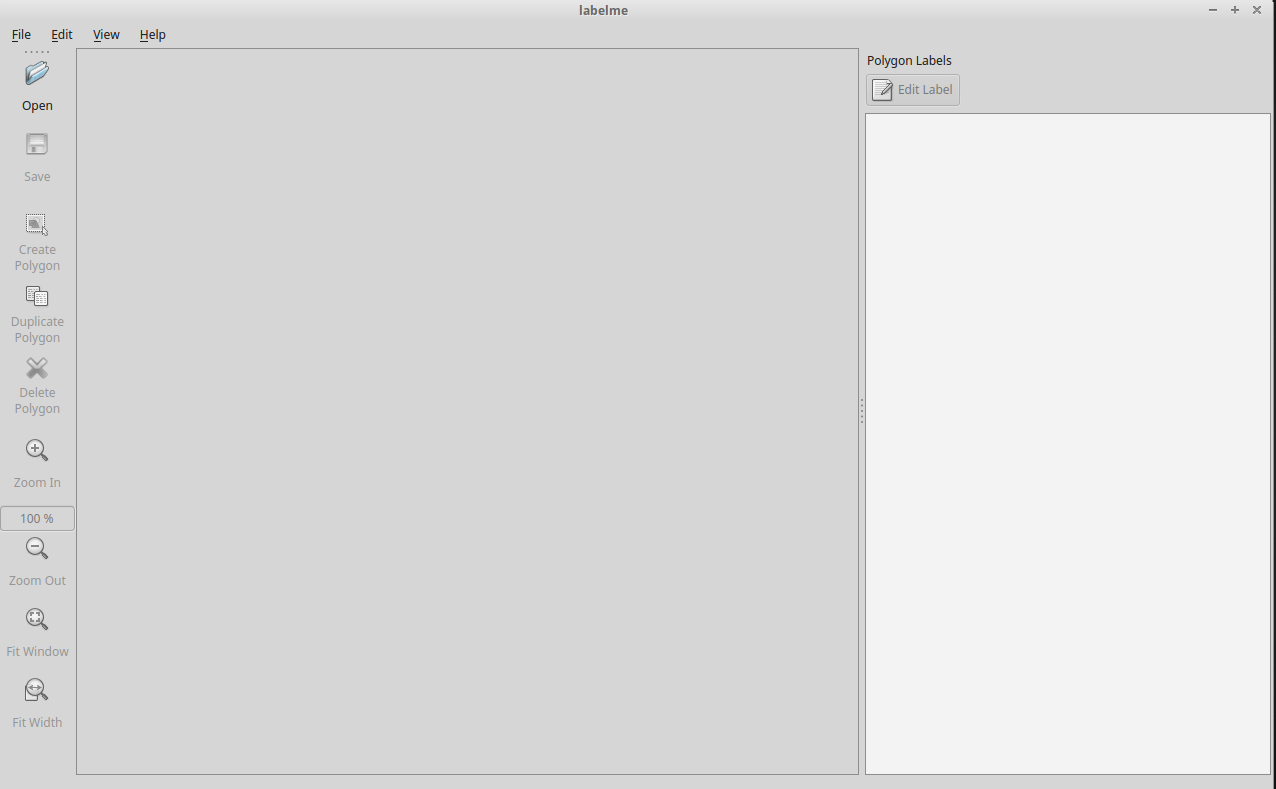
\includegraphics[height=9cm,keepaspectratio=true,clip=true]{imagenes/Logos/labelme.png}
  \caption{Pantalla Principal \textit{labelme}}
	\label{Fig: labelme}
\end{figure}

En las imágenes siguientes se muestra el proceso de anotación que se llevo a cabo mediante \textit{labelme}, para detalles de la instalación ir a: \ref{sec:instalacionlabelme}.

Cada anotación se almacena en un archivo .json que luego es transformado y almacenado en una tabla como vemos en \ref{tab:ejemGT}
\begin{figure}[h]
 \centering
  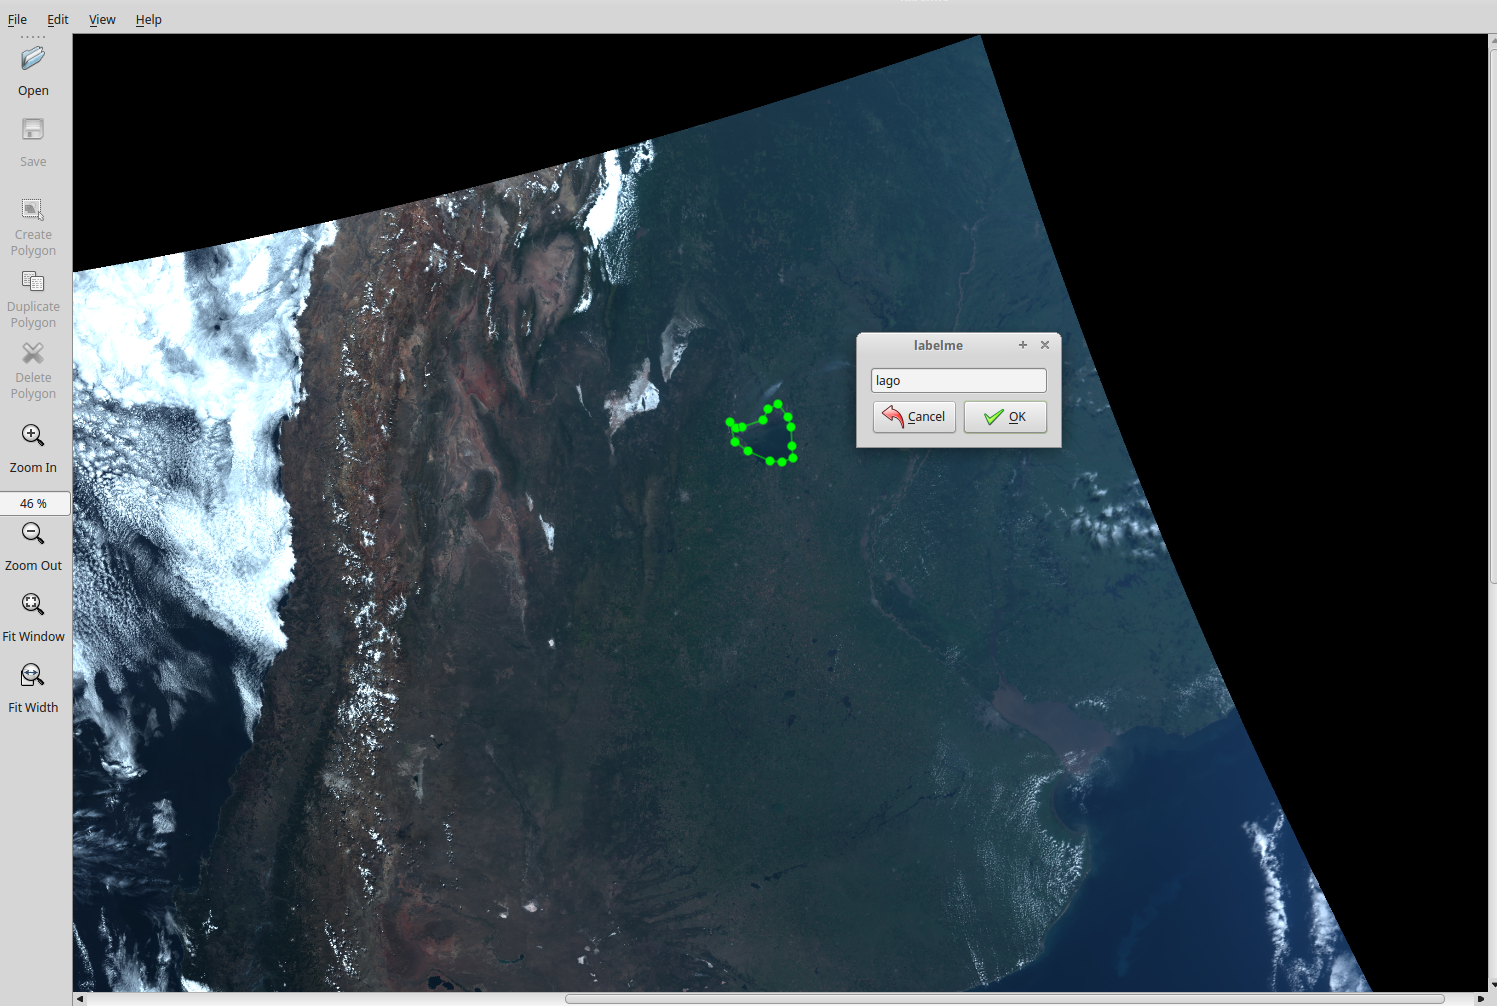
\includegraphics[height=8cm,keepaspectratio=true,clip=true]{imagenes/Logos/labelme1.png}
  \caption{Etiquetar una región en \textit{labelme}}
	\label{Fig: labelme1}
\end{figure}

\begin{figure}[H]
 \centering
  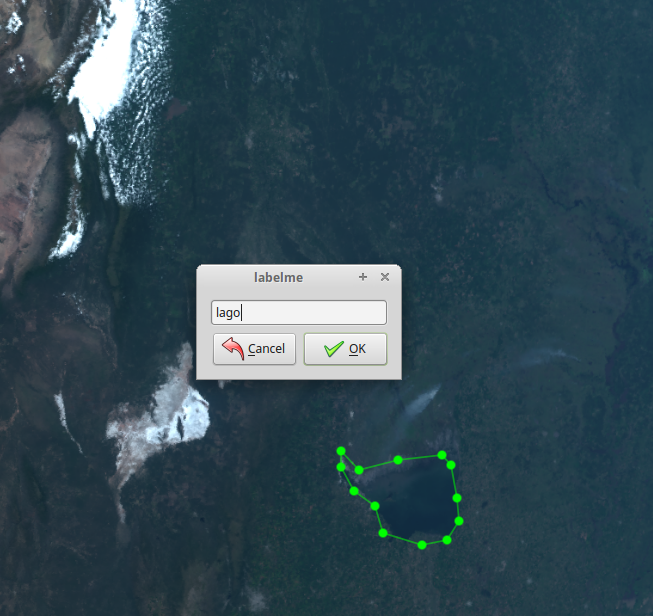
\includegraphics[height=10cm,keepaspectratio=true,clip=true]{imagenes/Logos/labelme2.png}
  \caption{Etiquetar una región en \textit{labelme}}
	\label{Fig: labelme2}
\end{figure}

El \textit{ground truth} final obtenido se guardo en el siguiente formato de anotación (ver \ref{tab:GT} y \ref{tab:ejemGT}):

\begin{table}[H]
\begin{center}
\begin{tabular}{|c|c|c|c|}
\hline Nombre & Bandas & Región & Puntos anotados(x,y)\\ \hline 
\end{tabular}
\end{center} \caption{Estructura ground truth.}\label{tab:GT}
\end{table}

\begin{table}[H]
\begin{center}
\begin{tabular}{|c|c|c|c|}
\hline \textbf{Nombre} & \textbf{Bandas} & \textbf{Región} & \textbf{Puntos anotados(x,y)}\\ \hline 
Imagen01 & 367 & Lago  & 23,50,55,22,223\\ \hline 
Imagen02 & 543 & Lago  & 55,26		\\ \hline 
Imagen03 & 543 & Golfo & 44,300,500,900 \\ \hline 
.......  & ...  & .....& ...............\\ \hline 
\end{tabular}
\end{center} \caption{Ejemplo ground truth.}\label{tab:ejemGT}
\end{table}


\subsection{Selección de Metodos Proposal}\label{sub:proposal}

Cada una de las imágenes obtenidas (ver: \ref{chap:recoleccion}), se aplico técnicas de selección de regiones candidatas para luego ser analizada y clasificada; para esta fase aplicamos métodos de \textit{Regions Proposal} visto en el capitulo \ref{chap:marcoteorico}.

La primera  consideración tomada fue analizar que método de \textit{Regions Proposal} se utilizaría. Se realizaron pruebas con los métodos \ac{bing}, Selective Search y Edge Boxes; donde podemos detallar lo siguiente: \ref{tabla:comparacionregiones}.

\begin{table}[H]
\centering
\begin{tabular}{|p{2cm}|p{6cm}|p{8cm}|}
    \hline 
     & \centering \textbf{Ventajas} & \multicolumn{1}{c|}{\centering \textbf{Desventajas}} \\
    \hline
    \centering Selective Search & \parbox[p][0.2\textwidth][c]{6cm}{
    \begin{itemize}
        \item Fácil implementación en python	
    \end{itemize}}  &  \parbox[p][0.2\textwidth][c]{7.5cm}{
    \begin{itemize}
        \item Tiempo de ejecución muy alto para imágenes de resolución mayores; ejemplo: 2800x3000px.	
    \end{itemize} } \\ \hline
    \centering Edges Boxes & \parbox[p][0.2\textwidth][c]{6cm}{
    \begin{itemize}
        \item Buen tiempo de ejecución con imágenes de gran tamaño
        \item Reconocimientos de regiones de menor tamaño
    \end{itemize} } & \parbox[p][0.2\textwidth][c]{7.5cm}{
    \begin{itemize}
        \item No se encontró una implementación optima en python.	
    \end{itemize} } \\ \hline 
     \centering BING & \parbox[p][0.2\textwidth][c]{6cm}{
    \begin{itemize}
        \item El tiempo de ejecución en imágenes de gran tamaño es optimo
    \end{itemize} } &  \parbox[p][0.2\textwidth][c]{7.5cm}{
    \begin{itemize}
        \item Baja probabilidad de encontrar regiones de menor tamaño en imágenes grandes.
    \end{itemize} } \\ \hline
\end{tabular}
\caption{Análisis de métodos Regiones Propuestas}
\label{tabla:comparacionregiones}
\end{table}

Unos de los principales inconvenientes a la hora del desarrollo de la tesis fue el tamaño de las imágenes. Las regiones de interés son mas pequeñas en proporción a la escala y tamaño de la imagen utilizada, por este motivo al aplicar técnicas de selección de candidatos no generalizaba de manera correcta las regiones que deseamos captar. Para eliminar este problema se procedió a realizar los siguientes pasos: 
\begin{enumerate}
 \item Para cada imagen original se corto en regiones de 256px de alto por el ancho total de la imagen (ver: \ref{Fig: cropimagen}), donde \textit{w} es el ancho de la imagen y \textit{h} alto de la imagen
 \item Se aplico para cada recorte obtenido el método \textit{Edges Boxes} para la obtención de regiones candidatas (ver: \ref{Fig: cropproposal}).

\begin{figure}[H]
 \centering
  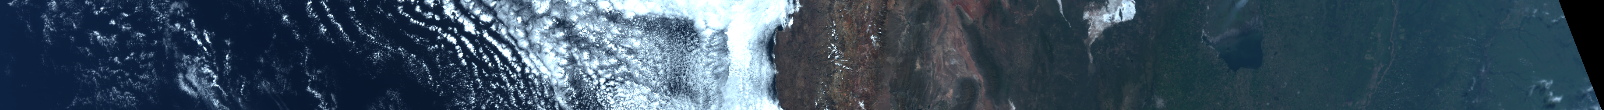
\includegraphics[height=1.2cm,keepaspectratio=true,clip=true]{imagenes/Logos/cropimagen.png}
  \caption{Crop de Imagen Satelital (4833\textit{w} X 256\textit{h})}
	\label{Fig: cropimagen}
\end{figure}

\begin{figure}[H]
 \centering
  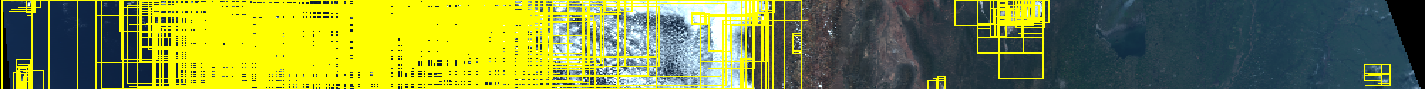
\includegraphics[height=1.1cm,keepaspectratio=true,clip=true]{imagenes/Logos/cropproposal.png}
  \caption{Aplicación de Edges Boxes a un recorte de la imagen.}
	\label{Fig: cropproposal}
\end{figure}

\item Para cada imagen se obtuvo 26 recortes en total, obteniendo el siguiente resultado en la imagen completa \ref{Fig: proposal}.

\begin{figure}[H]
 \centering
  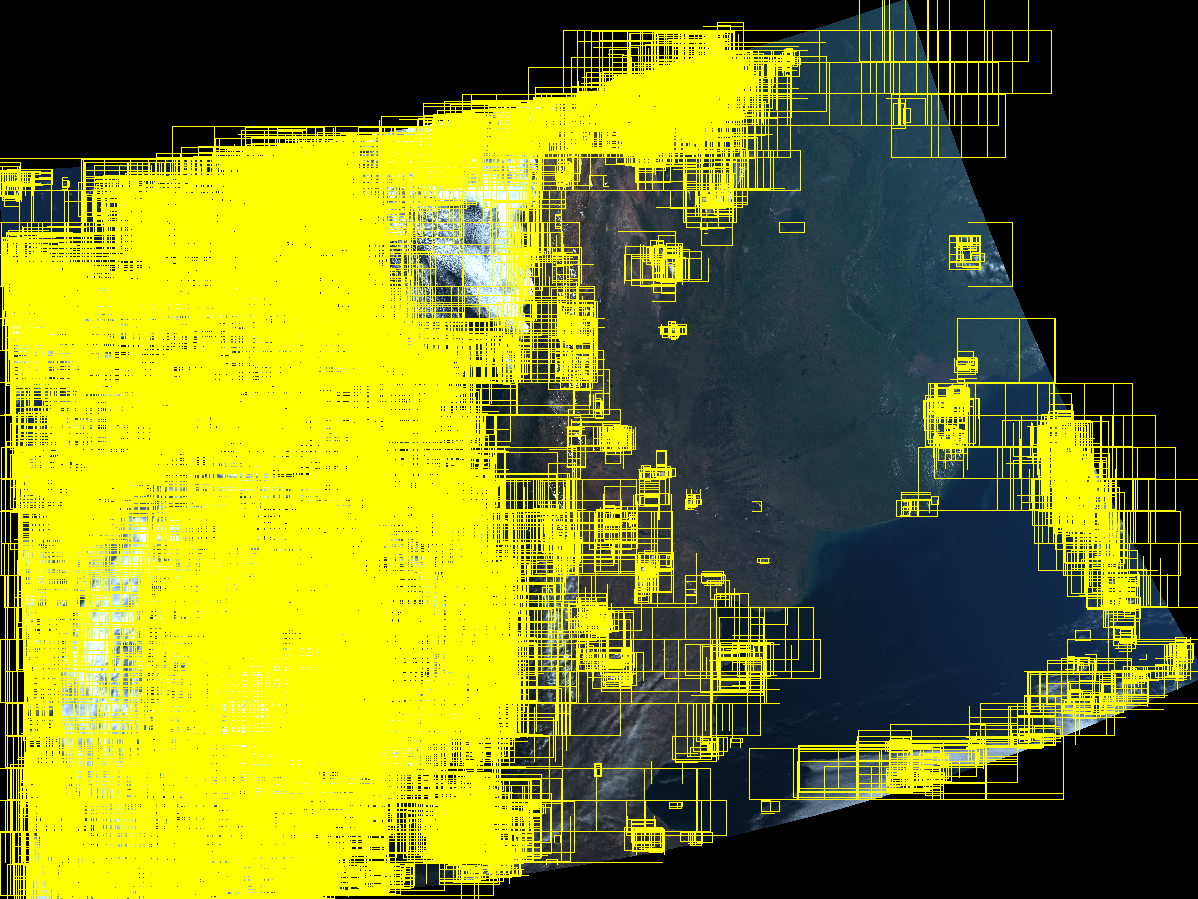
\includegraphics[height=13cm,keepaspectratio=true,clip=true]{imagenes/Logos/proposal.png}
  \caption{Aplicación de Regiones propuestas a una imagen satelital.}
	\label{Fig: proposal}
\end{figure}

\end{enumerate}
La imagen anterior \ref{Fig: proposal} se obtuvo 53.815 regiones por el método \textit{Edges Boxes} de selección de candidatos. Procesar estas 53.815 regiones candidatas consumirá mucho tiempo de computo, además podemos visualizar que existen regiones solapadas (overlapping); estas regiones representan información duplicada que debemos eliminar. 

Para solucionar el problema del \textit{overlapping}  aplicamos \ac{nms} visto en la sección \ref{sec:nonmaximumsuppression}. 
El valor usado para la eliminación de regiones candidatas duplicadas fue de 0.8 como valor de solapamiento entre regiones candidatas detectadas.

En la figura siguiente \ref{Fig: proposalnms} se pude observar que con un valor 0.8 de \textit{overlapping} aplicando \ac{nms} obtenemos un 90\% aproximadamente de optimización en la eliminación de regiones candidatas duplicada, es decir se paso de 53.815 a 1.560 regiones candidatas por imagen para el entrenamiento.

\begin{figure}[H]
 \centering
  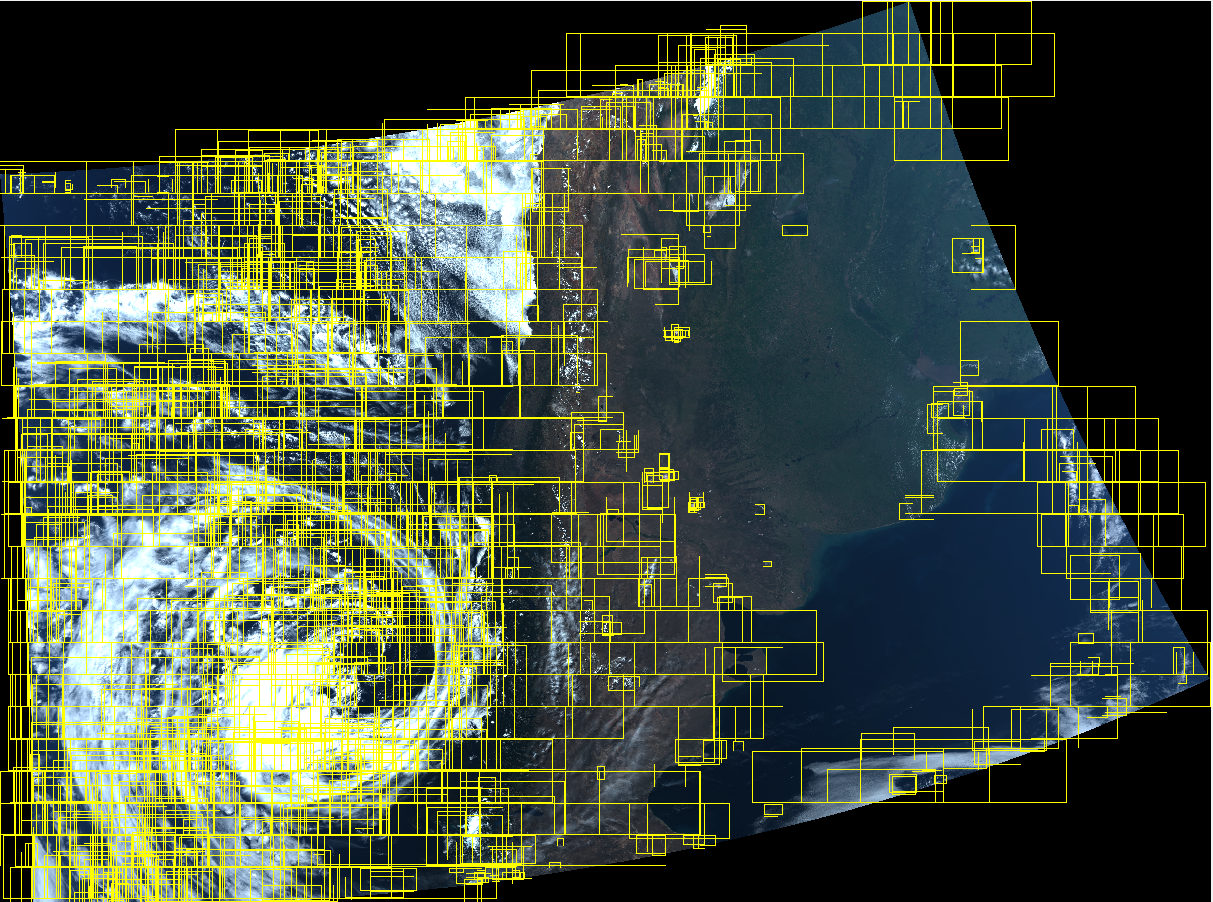
\includegraphics[height=13cm,keepaspectratio=true,clip=true]{imagenes/Logos/proposalconNMS.png}
  \caption{Proposal obtenido con Non-maximum suppression}
	\label{Fig: proposalnms}
\end{figure}


\subsection{Etiquetado de Regiones Candidatas}\label{sub:etiquetado}

Los datos obtenidos de la recolección de regiones candidatas a partir de los métodos \textit{Proposal} debe ser etiquetados para su entrenamiento. Para realizar el etiquetado se utilizo el \textit{ground truth} \ref{sub:groundtruth} que serán comparados con las regiones candidatas calculando el \textit{overlapping} entre estas.

El criterio utilizado en el etiquetado de datos es el siguiente:
\begin{enumerate}
	\item 0: NO contiene el patrón de interés en la región candidata.
	\item 1: Existencia del patrón en la región candidata.
\end{enumerate}

Para la selección de alguna de las etiquetas anteriores el umbral de decisión fue de 0.5 como valor de \textit{overlapping}, es decir el nivel de solapamiento que existen entre el \textit{ground truth} y la región candidata.


\section{Extracción de Características}\label{sec:extracciondecaracteristica}

En esta sección vamos a especificar el proceso de extracción  de característica realizado sobre una región. Para esto partiremos del los pasos desarrollados previamente \ref{sec:preprocesamiento}.

Calculando el método Edges Boxes y aplicando \ac{nms} vimos que obtuvimos aproximadamente 1560 regiones por imagen. A partir de estos datos calculamos el \textbf{\textit{feature vector}} que caracterice esa región; es decir para cada región encontrada debemos obtener un vector que represente de manera única esa región. Para la obtención del vector de característica se utilizo una \ac{cnn}. 

Los pasos que se siguieron para realizar esta tarea serán enumeramos a continuación:

\begin{enumerate}
	\item Para cada región propuesta de la imagen se realizo una escalamiento del tamaño de la región de interés y  transformando en una imagen de 256px x 256px.
	\item Cada imagen es una entrada a una \ac{cnn} que aplica en cada capa una operación matemática sobre la imagen.
	\item Se obtuvo la capa ante ultima de la red que contiene el \textit{feature vector} de la región. 
\end{enumerate}

El calculo del vector de característica, \textit{feature vector}, se utilizo la \ac{cnn} pre-entrenada \textbf{ResNet50}\footnote{Fuente: http://www.pyimagesearch.com/2017/03/20/imagenet-vggnet-resnet-inception-xception-keras/}. Esta red se basa en módulos de micro-arquitectura (también denominados arquitecturas de red en red). El término micro-arquitectura se refiere al conjunto de bloques utilizados para construir la red. Una colección de bloques de construcción de micro-arquitectura (junto con sus capas estándar CONV, POOL, etc.) conduce a la macro-arquitectura (es decir, a la propia red final). Para la obtención del vector de característica se extrajo la ante ultima capa de la red llamada \textit{\textbf{avg\_pool}}; esta capa retorna un vector de característica de 2048 elementos que representan la región.


Los datos se almacenaron en un archivo de extensión \textit{.mat}; que contiene los siguientes datos:
\begin{itemize}
 \item Las coordenadas de cada regiones candidatas.
 \item El \textit{feature vector} de 2048 elementos que corresponde a cada región. 
 \item Las etiquetas que indica a que clase pertenece la región; en este caso clasificación binaria (0 ó 1).
\end{itemize}





\section{Validación Experimental}\label{validacion}

A continuación se pondrá a disposición del lector los diversos experimentos realizados evaluando el comportamiento de los modelos de predicción obtenidos.

\subsection*{Conjunto de datos de Entrenamiento}

\textcolor{red}{Los experimentos se realizaron en base a XX imagenes; el datasets se dividió en tres conjuntos (test, validación y entrenamiento), para el conjunto de test se reservaron XX imágenes lo cual corresponde a 16\% de la muestra. Una ves excluidos los datos de test quedaron XX imágenes correspondiente al entrenamiento y validación en el  cual es el porcentaje restante 84\% de la muestra.  Cabe aclarar que cada imagen posee aproximadamente XXXX vectores de  característica, \textit{feature vector}; la cantidad de datos  para XX imágenes son de XXXXX vectores de característica para entrenamiento y validación. En cuanto  al conjunto de test son XXXX vectores de característica para las XX imágenes excluidas del entrenamiento.}

\textcolor{blue}{Además como se menciono en el capitulo \ref{chap:recoleccion} \ref{sec:datosutilizados}, se utilizo diferentes combinaciones de bandas para realizar validaciones del experimento. }

\subsection{Entrenamiento}\label{sub:entrenamiento}

Para realizar el entrenamiento de los datos se utilizo un clasificador \ac{svm} con kernel: \textit{linear y gaussiano \"RBF\"}. Como mencionamos previamente se dividió los datos en \textit{entrenamiento}, \textit{validación} y \textit{test}; para validar los datos de entrenamiento se uso \textit{cross-validation}, validación cruzada, dividiendo los datos de entrenamiento y validación en 5 conjuntos usando el algoritmo \textit{K-Folds}. 


\subsubsection{Parámetros}\label{sub:parametros}


Para obtener una predicción  correcta se debe optimizar algunos parámetros en el entrenamiento; para buscar los parámetros óptimos para la creación del modelo se realizaron pruebas con el algoritmo  \textit{\textbf{GridSearch}} y \textit{\textbf{RandomizeSearch}} \footnote{Fuente: https://goo.gl/koWr74} con \textit{k-folds}, contenido en la librería de \textit{Sklearn}\ref{sub:sklearn}, algoritmo que usa validación cruzada para la búsqueda. 


Los parámetros que permiten al clasificador minimizar el error en la predicción  son:
\begin{enumerate}
	\item \textbf{Parámetro C}: Controla el costo de la mala clasificación, \textit{misclassification}, en los datos de entrenamiento. Con un valor de C pequeño hará que el optimizador busque un hiperplano de separación de mayor margen, incluso si ese hiperplano clasifica erróneamente más puntos. Para valores muy pequeños de C, debe obtener ejemplos mal clasificados, a menudo incluso si sus datos de entrenamiento son linealmente separables. Para valores grandes de C,  elegirá un hiperplano de menor margen si ese hiperplano hace un mejor trabajo de conseguir que todos los puntos de entrenamiento estén clasificados correctamente. El objetivo es encontrar el equilibrio entre "no demasiado estricto" y "no demasiado relajado". La validación cruzada  son buenas maneras de encontrar el mejor C.

	\item \textbf{Parámetro gamma}: Es la inversa de la desviación estándar del kernel RBF (función gaussiana), que se utiliza como medida de similitud entre dos puntos. 
\end{enumerate}

Además de la optimización de los parámetros mencionados previamente, \textbf{C y gamma}, se  debe tener en cuenta las siguientes variables a la hora de evaluar un modelo: \textit{Accuracy, Precisión y Recall}. 

Las variables que intervienen en el calculo de \textit{Accuracy, Precisión y Recall} son:
\begin{itemize}
	\item Positivos (P): Observación positiva (valor etiquetado).
	\item Verdadero Positivo (TP): La observación es positiva y la predicción también.
	\item Falso Negativo (FN): La observación es positiva pero la predicción es negativa.
	\item Falso Positivo (FP): La observación es negativa pero la predicción es positiva.
	\item Verdadero Negativo (TN) :  La observación es negativa y también la predicción negativa.
\end{itemize}

\textbf{Accuracy:} Proporción de todas las predicciones que son correctas; da una medida de que tan bueno es el modelo.
\begin{equation}
accuracy = \frac{FP+FN}{FP+FN+TP+TN}=\frac{predicciones\;correctas}{todas\;las\;predicciones}
\end	{equation}
\textbf{Precisión:} Proporción de todas las predicciones positivas que son correctas. La precisión es una medida de cuántas predicciones positivas son reales.
\begin{equation}
precision=\frac{TP}{TP+FP}= \frac{predicciones\;correctamente\;positivas}{todas\;las\;predicciones\;positivas}
\end{equation}

\textbf{Recall:} Nos da la proporción de la observaciones reales positivas que son correcta, es decir nos da la precisión de cuantas observaciones positivas reales se obtuvo correctamente.
\begin{equation}
recall = \frac{TP}{TP+FN} = \frac{TP}{P} = \frac{predicciones\;a\;ser\;positiva}{todas\;la\;observaciones\;positivas} 
\end{equation}

El rango de parámetros usados para el entrenamiento y validación de datos fueron los siguientes:

\begin{itemize}
 \item \textbf{Valor de C}: 1000,100,10,1, 0.1,0.01,0.001,0.0001
 \item \textbf{Valor de Gamma}: 1,0,1,0,01,0,001,0,0001,0,00001
\end{itemize}



\subsection{Entrenamiento de Imágenes Bandas 5, 4 y 3 (True color)}\label{sub:entrenamiento_bandas543}

Cantidad de imágenes Train-val: 46 
Cantidad de imágenes Test : 16  

El total de feature vector para el entrenamiento:
\begin{itemize}
\item Tamaño del Train-val: 1361
\item Tamaño del Test: 356
\end{itemize}

Prueba con GridSearch conjunto Train-val, con validacion cruzada en 5 folds:

\begin{itemize}
\item Valores de \textit{Accuracy} (exactitud) optimo: \textbf{0.88221884498}
\item Valores de \textit{Kernel} optimo: \textbf{RBF}
\item Valores de \textit{C} optimo: \textbf{1000}
\item Valores de \textit{Gamma} optimo: \textbf{1}

\end{itemize}

Luego de obtener el modelo se realizo el test correspondiente obteniendo los siguientes valores:
\begin{table}[H]
\begin{center}
\begin{tabular}{|c|c|c|c|c|}
\hline \multicolumn{5}{|c|}{Reporte Test Entrenamiento} \\ \hline
\hline \textbf{} & \textbf{Precision} & \textbf{Recall} & \textbf{f1-score} & \textbf{Support}\\ \hline 
				 0   & 0.88 & 0.96 & 0.92  & 267	\\ \hline 
				 1   & 0.82 & 0.61 & 0.70  & 89 \\ \hline 
\textbf{avg / total} & 0.86 & 0.87 & 0.86  & 356 \\ \hline
\end{tabular}
\end{center} \caption{Test Entrenamiento bandas 5, 4, 3 con GridSearch}\label{tab:gridsearchtest543}
\end{table}


Prueba con RandomizeSearch conjunto Train-val, con validacion cruzada en 5 folds:

\begin{itemize}
\item Valores de \textit{Accuracy} (exactitud) optimo: \textbf{0.882218844985}
\item Valores de \textit{Kernel} optimo: \textbf{RBF}
\item Valores de \textit{C} optimo: \textbf{100}
\item Valores de \textit{Gamma} optimo: \textbf{1}

\end{itemize}

Luego de obtener el modelo se realizo el test correspondiente obteniendo los siguientes valores:
\begin{table}[H]
\begin{center}
\begin{tabular}{|c|c|c|c|c|}
\hline \multicolumn{5}{|c|}{Reporte Test Entrenamiento} \\ \hline
\hline \textbf{} & \textbf{Precision} & \textbf{Recall} & \textbf{f1-score} & \textbf{Support}\\ \hline 
				 0   & 0.88 & 0.96 & 0.92  & 267	\\ \hline 
				 1   & 0.82 & 0.61 & 0.70  & 89 \\ \hline 
\textbf{avg / total} & 0.86 & 0.87 & 0.86  & 356 \\ \hline
\end{tabular}
\end{center} \caption{Test Entrenamiento bandas 5, 4, 3 con RandomizeSearch}\label{tab:RandomTest543}
\end{table}


Prueba con Hard Negative Minning
Mejora en la exactitud, Accuracy: 0.884831460674



\subsection{Entrenamiento de Imágenes Bandas 10, 7 y 5}\label{sub:entrenamiento_bandas1075}

Cantidad de imágenes Train-val: 46 
Cantidad de imágenes Test : 16  

El total de feature vector para el entrenamiento:
\begin{itemize}
\item Tamaño del Train-val: 1584
\item Tamaño del Test: 536
\end{itemize}

Prueba con GridSearch conjunto Train-val, con validacion cruzada en 5 folds:

\begin{itemize}
\item Valores de \textit{Accuracy} (exactitud) optimo: \textbf{0.919823232323}
\item Valores de \textit{Kernel} optimo: \textbf{RBF}
\item Valores de \textit{C} optimo: \textbf{1000}
\item Valores de \textit{Gamma} optimo: \textbf{0.001}
\end{itemize}

Luego de obtener el modelo se realizo el test correspondiente obteniendo los siguientes valores:
\begin{table}[H]
\begin{center}
\begin{tabular}{|c|c|c|c|c|}
\hline \multicolumn{5}{|c|}{Reporte Test Entrenamiento} \\ \hline
\hline \textbf{} & \textbf{Precision} & \textbf{Recall} & \textbf{f1-score} & \textbf{Support}\\ \hline 
				 0   & 0.96 & 0.98 & 0.97  & 402	\\ \hline 
				 1   & 0.94 & 0.89 & 0.92  & 134 \\ \hline 
\textbf{avg / total} & 0.96 & 0.96 & 0.96  & 536 \\ \hline
\end{tabular}
\end{center} \caption{Test Entrenamiento bandas 10, 7, 5 con GridSearch}\label{tab:gridsearchtest1075}
\end{table}


Prueba con RandomizeSearch conjunto Train-val, con validacion cruzada en 5 folds cada 10 candidatos:

\begin{itemize}
\item Valores de \textit{Accuracy} (exactitud) optimo: \textbf{0.919823232323}
\item Valores de \textit{Kernel} optimo: \textbf{RBF}
\item Valores de \textit{C} optimo: \textbf{10} 	
\item Valores de \textit{Gamma} optimo: \textbf{0.1}

\end{itemize}

Luego de obtener el modelo se realizo el test correspondiente obteniendo los siguientes valores:
\begin{table}[H]
\begin{center}
\begin{tabular}{|c|c|c|c|c|}
\hline \multicolumn{5}{|c|}{Reporte Test Entrenamiento} \\ \hline
\hline \textbf{} & \textbf{Precision} & \textbf{Recall} & \textbf{f1-score} & \textbf{Support}\\ \hline 
				 0   & 0.96 & 0.98 & 0.97  & 402	\\ \hline 
				 1   & 0.94 & 0.88  & 0.91 & 134 \\ \hline 
\textbf{avg / total} & 0.96 & 0.96 & 0.96  & 536 \\ \hline
\end{tabular}
\end{center} \caption{Test Entrenamiento bandas 5, 4, 3 con RandomizeSearch}\label{tab:RandomTest1075}
\end{table}


Prueba con Hard Negative Minning
Mejora en la exactitud, Accuracy: 0.960820895522



\subsection{Entrenamiento de Imágenes Bandas 11, 12 y 13}\label{sub:entrenamiento_bandas1111213}

Cantidad de imágenes Train-val: 46 
Cantidad de imágenes Test : 16  

El total de feature vector para el entrenamiento:
\begin{itemize}
\item Tamaño del Train-val: 1744
\item Tamaño del Test: 556
\end{itemize}

Prueba con GridSearch conjunto Train-val, con validacion cruzada en 5 folds:

\begin{itemize}
\item Valores de \textit{Accuracy} (exactitud) optimo: \textbf{0.872133027523}
\item Valores de \textit{Kernel} optimo: \textbf{RBF}
\item Valores de \textit{C} optimo: \textbf{1000}
\item Valores de \textit{Gamma} optimo: \textbf{1}
\end{itemize}

Luego de obtener el modelo se realizo el test correspondiente obteniendo los siguientes valores:
\begin{table}[H]
\begin{center}
\begin{tabular}{|c|c|c|c|c|}
\hline \multicolumn{5}{|c|}{Reporte Test Entrenamiento} \\ \hline
\hline \textbf{} & \textbf{Precision} & \textbf{Recall} & \textbf{f1-score} & \textbf{Support}\\ \hline 
				 0   & 0.90 & 0.99 & 0.94  & 417	\\ \hline 
				 1   & 0.95 & 0.68 & 0.79  & 139 \\ \hline 
\textbf{avg / total} & 0.92 & 0.91 & 0.91  & 556 \\ \hline
\end{tabular}
\end{center} \caption{Test Entrenamiento bandas 11, 12,13 con GridSearch}\label{tab:gridsearchtest111213}
\end{table}


Prueba con RandomizeSearch conjunto Train-val, con validacion cruzada en 5 folds cada 10 candidatos:

\begin{itemize}
\item Valores de \textit{Accuracy} (exactitud) optimo: \textbf{0.860091743119}
\item Valores de \textit{Kernel} optimo: \textbf{RBF}
\item Valores de \textit{C} optimo: \textbf{1000} 	
\item Valores de \textit{Gamma} optimo: \textbf{0.1}

\end{itemize}

Luego de obtener el modelo se realizo el test correspondiente obteniendo los siguientes valores:
\begin{table}[H]
\begin{center}
\begin{tabular}{|c|c|c|c|c|}
\hline \multicolumn{5}{|c|}{Reporte Test Entrenamiento} \\ \hline
\hline \textbf{} & \textbf{Precision} & \textbf{Recall} & \textbf{f1-score} & \textbf{Support}\\ \hline 
				 0   & 0.89 & 0.98 & 0.93  & 417	\\ \hline 
				 1   & 0.91 & 0.64  & 0.75 & 139 \\ \hline 
\textbf{avg / total} & 0.90 & 0.89 & 0.89  & 556 \\ \hline
\end{tabular}
\end{center} \caption{Test Entrenamiento bandas 11, 12, 13 con RandomizeSearch}\label{tab:RandomTest111213}
\end{table}


Prueba con Hard Negative Minning
Mejora en la exactitud, Accuracy: 0.911870503597





\textcolor{red}{\subsection{Modelos de Entrenamiento SVM}\label{sub:linealModel}}

La manera mas básica de usar un clasificador \ac{svm} es por medio de un kernel lineal, es decir crear una frontera de decisión a partir de una línea 
recta. 

%\subsection{Modelo RBF}\label{sub:RBFModel}
Un modelo RBF , \textit{Radial basis function}, es un kernel muy utilizado en la clasificación en reconocimiento de patrones; esta dada por la siguiente ecuación:
\begin{equation}
K(x,x')=\exp(-\frac{ \|x-x'\|^2}{2\sigma^2} )
\end{equation}\label{ec: ecuacionrbf}
En el cual \(\|x-x'\|\) es la distancia euclidiana cuadrada entre dos puntos de datos \(x\) y \(x'\)






\textcolor{red}{\subsection{Hard Negative Mining}\label{sub:hardnegativemining}}

Luego de buscar los parámetros óptimos para el modelo, el paso siguiente es el entrenamiento nuevamente de un modelo con los parámetros previamente obtenidos a partir de \textbf{GridSearch} o \textbf{RandomizeSearch}.

Para lograr una mayor precisión en el modelo de dato aplicamos la técnica \textit{hard negative mininig}, esta técnica nos permite eliminar los falsos positivos arrojados por el modelo.

Los pasos que se utilizaron son los siguientes:
\begin{enumerate}
	\item Entreno el clasificador con los valores óptimos obtenido.
	\item En base al conjunto de test obtengo solo los datos que tengan etiqueta negativa.
	\item Calculo la predicción de esos datos en base al clasificador entrenado.
	\item Si la predicción retorna algún valor = 1(\"positivo\"), guardo ese valor y lo agrego al conjunto train-val
	\item Retorno al paso 1; esto lo realizo 5 veces.
	\item Calculo el valor de Accuracy en base al ultimo modelo obtenido de las iteraciones.
\end{enumerate}

\begin{figure}[H]
 \centering
  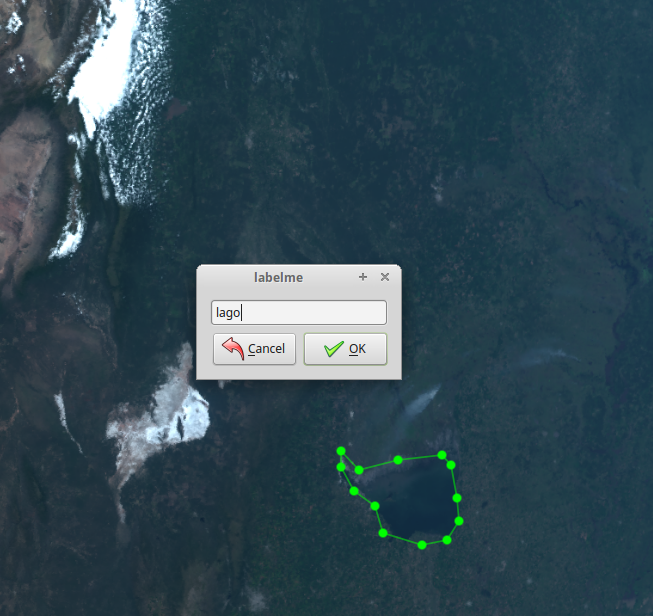
\includegraphics[height=10cm,keepaspectratio=true,clip=true]{imagenes/Logos/labelme2.png}
  \caption{Reconocimiento de Patrones (Golfo San Matias, Mar Chiquita)}
	\label{Fig: reconocimientopatrones}
\end{figure}



